\chapter{Methodology} % Main chapter title

\label{Methodology} % For referencing the chapter elsewhere, use \ref{Chapter2}




\section{Dataset Evaluation}


\begin{marginfigure}[-5\baselineskip] % move figure up by 1 line 
    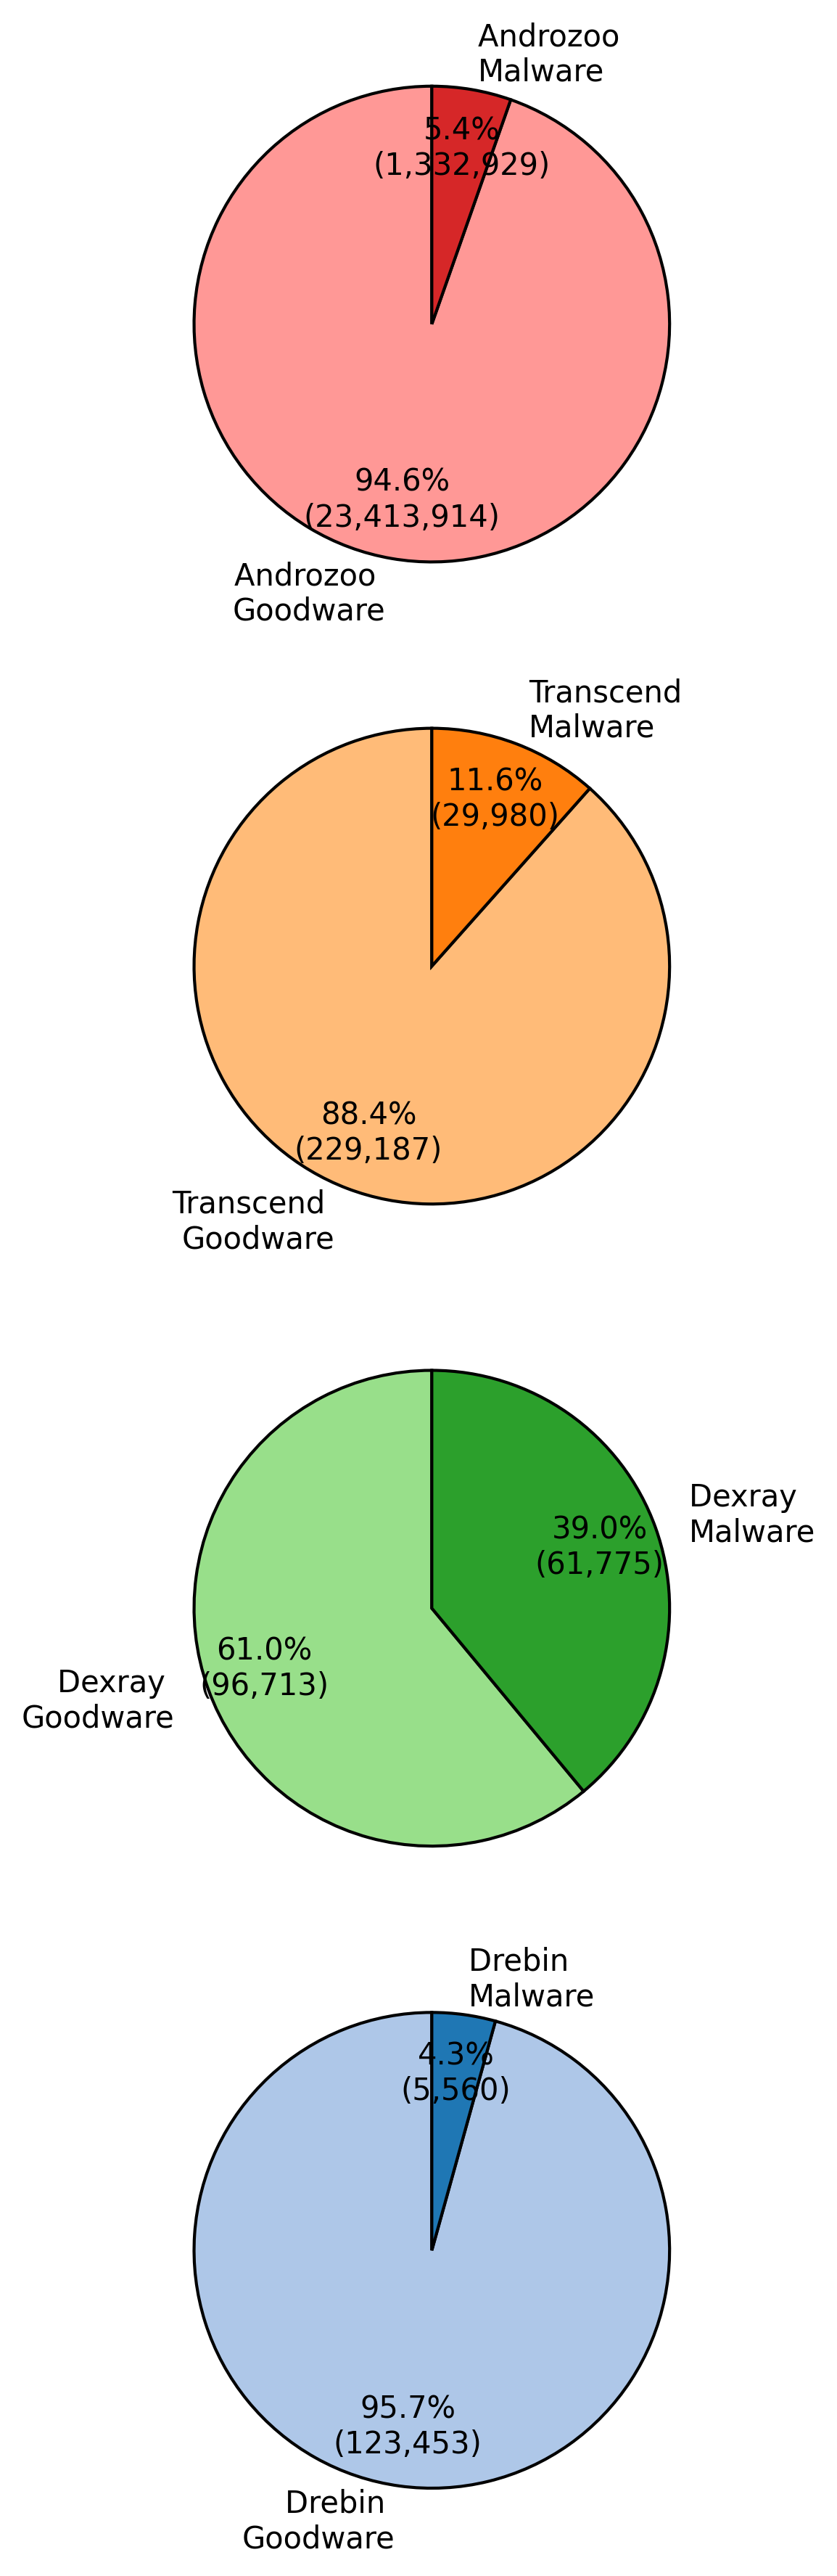
\includegraphics[width=1\marginparwidth]{3_Methodology/malware_goodware_ratios.png}
    \caption{\label{fig:marfig}The Malware to Goodware ratio of each analyzed Dataset shown as Pie Charts.}
\end{marginfigure}

There are mutiple available Datasets for Static Android Malware Detection.
Arp et al introduced 2014 the Drebin Dataset, this dataset has been used alot in the field. It consists of 

\subsection{Temporal Evaluation}

\section{Testbed Definition}

\section{Baseline Creation}

\subsection{Drebin}

\subsection{DetectBERT}

\section{Experimntal Setup}

\subsection{Android App Representaion}

\subsection{Model Implementation}

